\documentclass[lang=cn,10pt,newtx]{elegantbook}

\title{ElegantBook:优美的 \LaTeX{} 书籍模板}
\subtitle{Elegant\LaTeX{} 经典之作}

\author{Ethan Deng \& Liam Huang}
\institute{Elegant\LaTeX{} Program}
\date{Aug 15, 2022}
\version{4.4}
\bioinfo{自定义}{信息}

\extrainfo{要让一群人团结起来,需要的不是英明的领导,而是共同的敌人。—— 比企谷八幡}

\setcounter{tocdepth}{3}

\logo{logo-blue.png}
\cover{cover.jpg}

% 本文档命令
\usepackage{array}
\newcommand{\ccr}[1]{\makecell{{\color{#1}\rule{1cm}{1cm}}}}

% 修改标题页的橙色带
\definecolor{customcolor}{RGB}{32,178,170}
\colorlet{coverlinecolor}{customcolor}
\usepackage{cprotect}

\addbibresource[location=local]{reference.bib} % 参考文献,不要删除

\begin{document}

\maketitle
\frontmatter

\tableofcontents

\mainmatter

\chapter{Elegant\LaTeX{} 系列模板介绍}


\section{Gnuplot 绘图工具}
这是自己早期经常用的绘图工具,现在已经完全用Python实现,不再使用。

\subsection{安装}
(一)

注意不要直接安装,即\verb*|sudo apt-get install gnuplot|,通常缺少一个外界的库,容易造成terminal set to unknown错误,进而不能显示绘制图片。采用以下命令安装:

\verb*|sudo apt-get install gnuplot-x11|

或者分两步安装

\verb*|sudo apt-get install libx11-dev|

\verb*|sudo apt-get install gnuplot|



(二)源代码编译安装
\begin{itemize}
\item 先执行\verb*|sudo apt-get install libx11-dev|  安装x11,否则不能显示图形!\\
若不安装,则会出现,在终端下输入gnuplot后显示terminal set to unknown。

\item 去官网下载gnuplot版本并解压

\item \verb*|su root|

\item 切换到gnuplot所在目录

\item 配置\verb*|./configure|

\item 编译 make

\item  make install

\item 运行:在终端输入 gnuplot 就行了

\item 例子: plot sin(x)
\end{itemize}



\subsection{文件设置}
\subsubsection{设置数据分隔符}
%http://blog.csdn.net/liyuanbhu/article/details/8516417
\begin{verbatim}
set datafile separator ","
#设置gnuplot读取逗号分隔的数据文件
\end{verbatim}

有时,我们的数据文件中各个数据之间是用逗号作为分隔符的,比如标准的以“CSV”(Comma-Separated Values)为后缀的数据文件。如果在逗号之后没有空格分隔,默认情况下gnuplot是无法直接读取的。这时可以有两种方案,第一种是提前处理一下数据文件,比如将逗号替换为空格,随便一个文本处理软件都能很轻松的做这种替换。但是有时我们有很多这样的数据文件,每个都这样处理一下也挺麻烦的。第二种方法就是在gnuplot中给出文件分隔符的信息,让gnuplot能够读懂我们的文件。

例如:

\verb*|Plot 'sample.csv' using 1:2|

gnuplot 会抱怨说:
\begin{verbatim}
gnuplot> plot 'sample.csv' using 1:2
                                   ^
         warning: Skipping data file with no valid points
                                    ^
         x range is invalid
\end{verbatim}

正确的方法是这样的:

\verb*|plot 'sample.csv' using 1:2 "%lf,%lf"|

格式字符串的格式与C语言中scanf的格式字符串是类似的,实际上gnuplot就是用的scanf函数来读取数据。\verb|%lf| 
表示按照 double型浮点数类型来读取。需要注意的是gnuplot的格式化字符串不支持\verb|%lf| 。
gnuplot的格式化字符串还有很多的用法,这里就不多介绍了,有兴趣的可以参考帮助文档相关章节。

更一般的参考说明文档
\begin{verbatim}
Set datafile separator
The command set datafile separator tells gnuplot that data fields in subsequent input files are separated
by a specific character rather than by whitespace. The most common use is to read in csv (comma-separated
value) files written by spreadsheet or database programs. By default data fields are separated by whitespace.
Syntax:
set datafile separator {whitespace | tab | comma | "<chars>"}
Examples:
# Input file contains tab-separated fields
set datafile separator "\t"
# Input file contains comma-separated values fields
set datafile separator comma
# Input file contains fields separated by either * or |
set datafile separator "*|"
\end{verbatim}


\subsubsection{重命名数据文件}
\begin{verbatim}
datafile = "FMO-sink-initial1.ods"
#将数据文件命名为“datafile”,方便调用
\end{verbatim}



\subsection{图片设置}
\subsubsection{设置输出图片格式和名称}
\begin{verbatim}
set term post eps color enh solid
#设置输出图片格式
set output "FMO-sink-initial1.eps"
#设置输出图片名称
\end{verbatim}

其他图片格式的,有
\begin{itemize}
\item PS格式:
彩色(推荐使用):
\begin{verbatim}
set term postscript enhanced color
set output "*.ps"
\end{verbatim}
另:(未测)
\begin{verbatim}
set term postscript landscape
set output "*.ps"
\end{verbatim}

\item EPS格式:
黑白(曲线类型控制未知):
\begin{verbatim}
set term postscript eps enhanced
set output "*.eps"
\end{verbatim}
忘了是啥:
\begin{verbatim}
set term post eps color solid enh
set output "*.eps"
\end{verbatim}

\item PNG格式:
\begin{verbatim}
set terminal png size 1500,1000 enhanced font "Helvetica,20"
set output '*.png'
\end{verbatim}

\item PDF格式需要装有ps2pdf,然后:
\begin{verbatim}
set term postscript enhanced color
set output "| ps2pdf - *.pdf"
\end{verbatim}

注:关于pdf图片,输出后周围的大片空白可以在终端中使用如下命令去除:
pdfcrop *.pdf
会生成一个新文件: *-crop.pdf
使用此pdf文件在Latex等处都将十分整洁方便,妈妈再也不用担心我的图片了。
\end{itemize}


\subsubsection{设置图片/字体大小}
\begin{verbatim}
set size 1.0,1.0
#设置图片大小
\end{verbatim}
字体大小设置比较复杂,此命令是按比例缩放图片大小,字体大小不变,相当于字体相对变大。


\subsubsection{设置图片标题}
 设置/取消命名(位于图上方)
 \begin{verbatim}
set title "figurename""
unset title
\end{verbatim}
注:在多图设置(见8小节)中,命名命令对其后所有图生效,要在每个图中重新命名。之后不需要命名时要记得取消。


\subsubsection{设置图注}
\begin{enumerate}
\item 图注在图中的位置:
\verb*|set key left/right top/bottom/center|

\item 图注增加/取消外框:\verb*|set/unset key box|

\item 图注间距:\verb*|set key spacing 1.5|

\item 图注位于图外:\verb*|set key lmargin/rmargin/tmargin/bmargin(below)|

\item 取消图注:\verb*|unset key|
\end{enumerate}

图注设置参数一览:
\begin{verbatim}
set key {on|off} {default}
             {{inside | outside} | {lmargin | rmargin | tmargin | bmargin}
               | {at <position>}}
             {left | right | center} {top | bottom | center}
             {vertical | horizontal} {Left | Right}
             {{no}reverse} {{no}invert}
             {samplen <sample_length>} {spacing <vertical_spacing>}
             {width <width_increment>}
             {height <height_increment>}
             {{no}autotitle {columnheader}}
             {title "<text>"} {{no}enhanced}
             {{no}box { {linestyle | ls <line_style>}
                        | {linetype | lt <line_type>}
                          {linewidth | lw <line_width>}}}
     unset key
     show key
\end{verbatim}



\subsection{坐标轴设置}
\subsubsection{设置/取消坐标名称}
 \begin{verbatim}
set xlabel/ylabel "name"
unset xlabel/ylabel
\end{verbatim}


\subsubsection{设置坐标轴范围}
\begin{itemize}
\item 设置给定坐标轴范围\\
\verb|set xrange/yrange [1:100]|

\item 设置负向坐标
\verb|set xrange/yrange [100:1]|

\item 只设置一端坐标(另一端将自动调整)\\
\verb|set xrange/yrange [:100]|

\item 恢复自动坐标轴范围(此时人工给定设置依然保留)\\
\verb|set auto x/y|

\item  恢复给定坐标轴范围\\
\verb|set noauto x/y|
\end{itemize}

注:坐标轴范围,可以不设置,自动判断



\subsubsection{设置坐标轴标识}
\begin{itemize}
\item 设置坐标轴最大间隔(显示数值)\\
\verb|set xtics/ytics 0.5|

\item 设置坐标轴小间隔\\
\verb|set mxtics/mytics 2|\\
说明:将每个大间隔平分为2份

\item 设置坐标轴刻度的精度\\
\verb|set xtics format "%.2f"|\\
\verb|set ytics format "%.0f"|\\
说明:“\%.2f”指的是浮点型、精确到小数点后两位

\item 设置标识文本显示倾斜度\\
\verb|set xtics rotate by -45|\\
说明:标识右倾45度

\item 设置指数坐标轴\\
\verb|set log x/y|\\
\verb|set xtics 1.5|\\
说明:设置指数坐标轴的间隔时,数字代表10的指数(待明)。注意此时坐标的值域必须大于0。

\item 移动坐标标记\\
\verb|set x/ytics [out] offset 1,1|\\
“1,1” 为对应的移动向量的x,y值。
\end{itemize}



\subsection{代码示例}
\subsubsection{一维绘图图}
\lstinputlisting[language=gnuplot]{program/gnuplot/plot_1d.sh}
效果如下:
\begin{figure}[htb]
\centering
\includegraphics[width=0.7\textwidth]{program/gnuplot/diagonal.eps}
%\caption{精确解、欧拉法解、改进欧拉法解}
%\label{fig:by:table}
\end{figure}



\subsubsection{二维三维绘图}
给数据加入空白行Shell脚本:
\lstinputlisting[language=sh]{program/gnuplot/addblanks.awk}
二维等高图代码:
\lstinputlisting[language=gnuplot]{program/gnuplot/2d_contour.sh}
三维绘图代码:
\begin{lstlisting}[language=gnuplot]
#==================Pm3d绘图====================#
unset key
#pm3d绘图时,NxM的数据只能画出(N-1)x(M-1)的图像
set pm3d
#用色彩来表示不同的z值,palette-mapped 3d.
set palette rgbformulae 22,13,-31
#设置色板
replot

set pm3d at bs
#色彩图除了画在曲面上,还可以画在底部或顶部。b,s,t 三个字母分别代表底部、曲面和顶部,at 之后可以是任一个字母,也可是三个字母的任意组合。
replot
#splot datafile with lines

set pm3d map
#从上往下看数据
set size square
replot


#=================Image绘图===================#
set size square
plot datafile with image
#Image绘图与Pm3d绘图这两种方式无法简单判断优劣,只能根据实际需要选择。当像素比较多而数据又比较平滑的时候,其实两者差别不大。
\end{lstlisting}


效果如下:

%\begin{figure}[htb]
%\centering
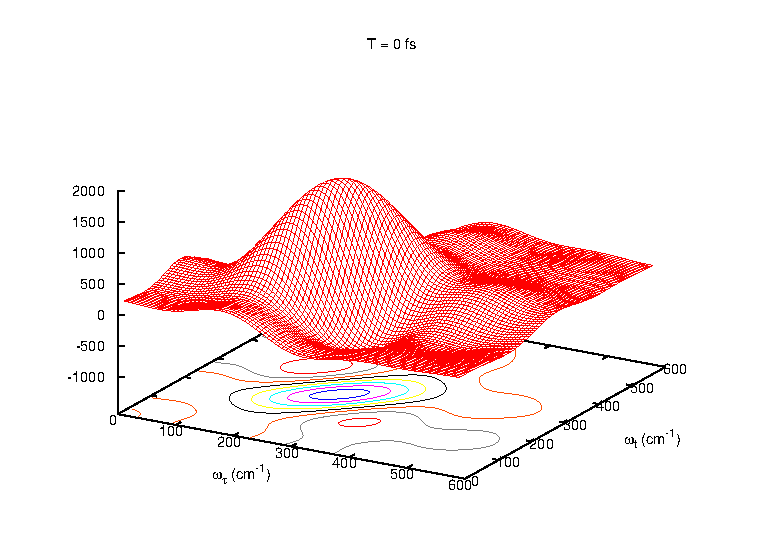
\includegraphics[width=0.4\textwidth]{program/gnuplot/re_rp1.eps}
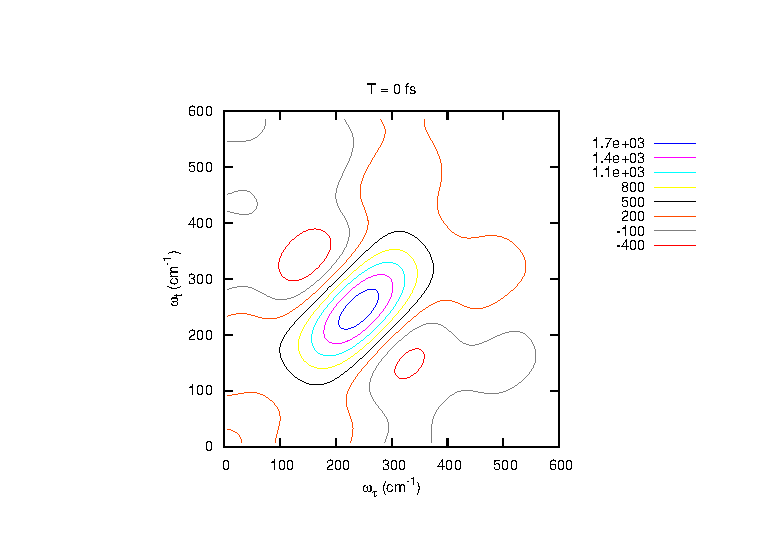
\includegraphics[width=0.4\textwidth]{program/gnuplot/re_rp2.eps}

\includegraphics[width=0.7\textwidth]{program/gnuplot/re_rp3.eps}

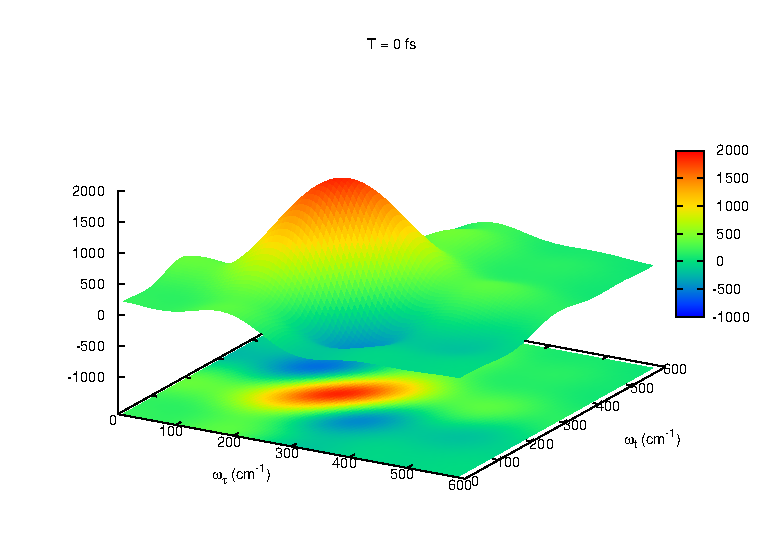
\includegraphics[width=0.7\textwidth]{program/gnuplot/re_rp4.eps}
%\caption{精确解、欧拉法解、改进欧拉法解}
%\label{fig:by:table}
%\end{figure}




\end{document}
